\hypertarget{Autoware Deployment Results}{%
\section{Autoware Deployment Results}\label{Autoware Deployment Results}}

The two of us worked with the Autoware stack for the very first time while operating and experimenting with the OpenCAV at CU-ICAR. This full-scale modular, open-architecture, open-interface, and open-source-software-based research instrument gave us ample opportunity to look ``under the hood'' and understand how this complex system-of-systems functions autonomously.

Furthermore, the format of the operational demo of OpenCAV shuttle rides across CU-ICAR campus motivated us to define the exact problem statement for the Autoware-based autonomy deployment segment of the project. This end-to-end autonomy pipeline works in 3 stages.

\begin{enumerate}
    \item First, the environment is mapped using the LIDAR point cloud data and optionally using odometry estimates by fusing IMU and encoder data while driving (or teleoperating) the vehicle manually.
    \item Next, a reference trajectory is generated by manually driving the vehicle within the (pre)mapped environment, while recording the waypoint coordinates as the vehicle localization estimates space a certain threshold distance apart with respect to the map's coordinate frame (using the LIDAR point cloud data and optionally using odometry estimates by fusing IMU and encoder data). It is worth mentioning that a reference trajectory can also be defined completely offline by using the map information alone, however, in such a scenario, proper care needs to be taken to ensure that the resulting trajectory is completely safe and kinodynamically feasible for the vehicle to follow in autonomous mode.
    \item Finally, in autonomous mode, the vehicle tracks the reference trajectory using a linearized pure-pursuit controller for lateral motion control and PID controller for longitudinal motion control.
\end{enumerate}

The exact inputs, outputs, and configurations of perception, planning, and control modules vary with the underlying vehicle platform. Therefore, to keep the overall project clean and well-organized, a multitude of custom meta-packages were developed within the Autoware Universe stack to handle different perception, planning, and control algorithms using different input and output information in the form of independent individual packages.

Additionally, a separate meta-package was created to handle different vehicles of the AutoDRIVE Ecosystem exploited in this project viz. Nigel, F1TENTH, Hunter SE and OpenCAV. Each package for a particular vehicle hosts vehicle-specific parameter description configuration files for perception, planning, and control algorithms, map files, RViz configuration files, API program files, teleoperation program files, and user-convenient launch files for getting started quickly and easily.

It is worth mentioning that we have also implemented a couple of high-level system configurations within the Autoware stack to ensure proper operation of the autonomous vehicles.

\begin{enumerate}
    \item A trajectory looping criteria to determine if the very first waypoint in the reference trajectory is to be set as the target waypoint for the controller upon successful tracking of the very last waypoint in the reference trajectory. This helps effectively shape a “safe termination” behavior for the ego vehicle upon the end of the reference trajectory, which is extremely important in certain applications (e.g. autonomous valet parking) as discussed in further sections. Furthermore, the tolerance on the termination criteria helps the ego vehicle come to a safe stop smoothly without any unnecessarily aggressive over-corrections or any overshoots outside the safe space.
    \item An operational control mode for the vehicle to engage the ego vehicle selectively in a simplistic gym environment, high-fidelity simulation environment, purely testbed (real-world hardware) mode, or in a true digital twin framework exploiting the high-fidelity simulator in conjunction with the testbed.
\end{enumerate}

\hypertarget{F1TENTH}{%
\subsection{F1TENTH}\label{F1TENTH}}

\begin{figure}[H]
    \centering
    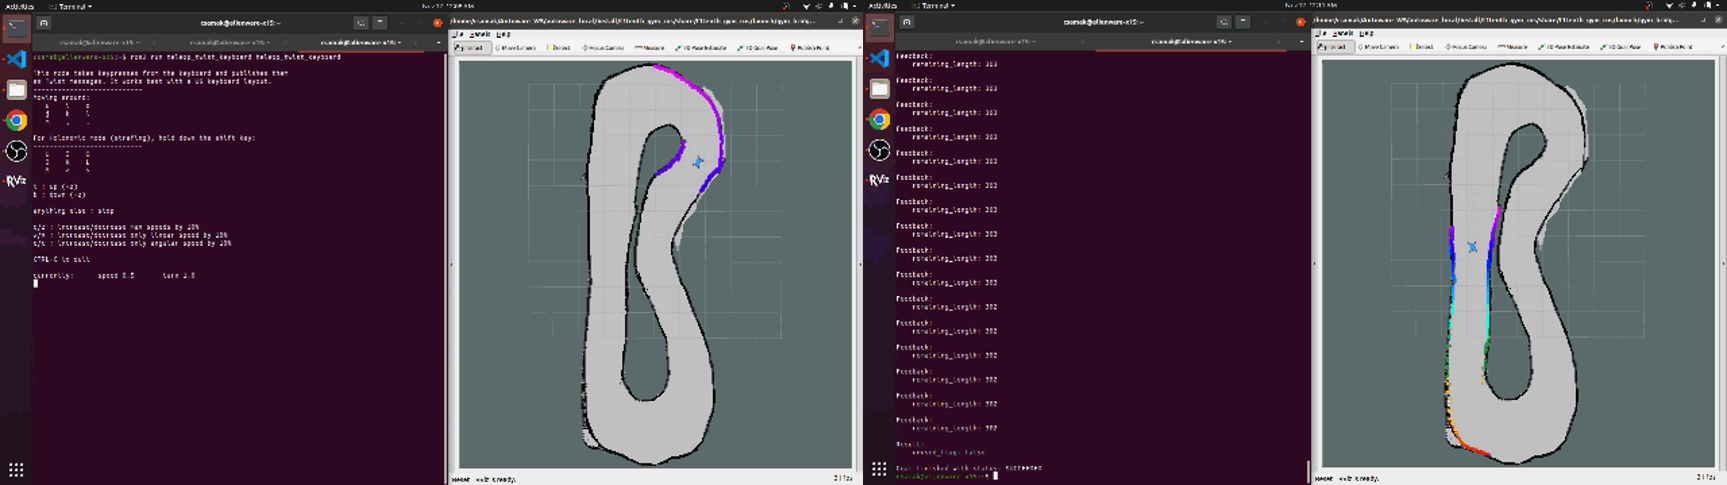
\includegraphics[width=\linewidth]{Figures/fig12.png}
    \caption{AutoDRIVE-F1TENTH-Autoware integration for autonomous racing ODD: RViz Gym demo for recording a trajectory using manual teleoperation and then tracking the pre-recorded trajectory autonomously.}
    \label{fig: figure12}
\end{figure}

\begin{figure}[H]
    \centering
    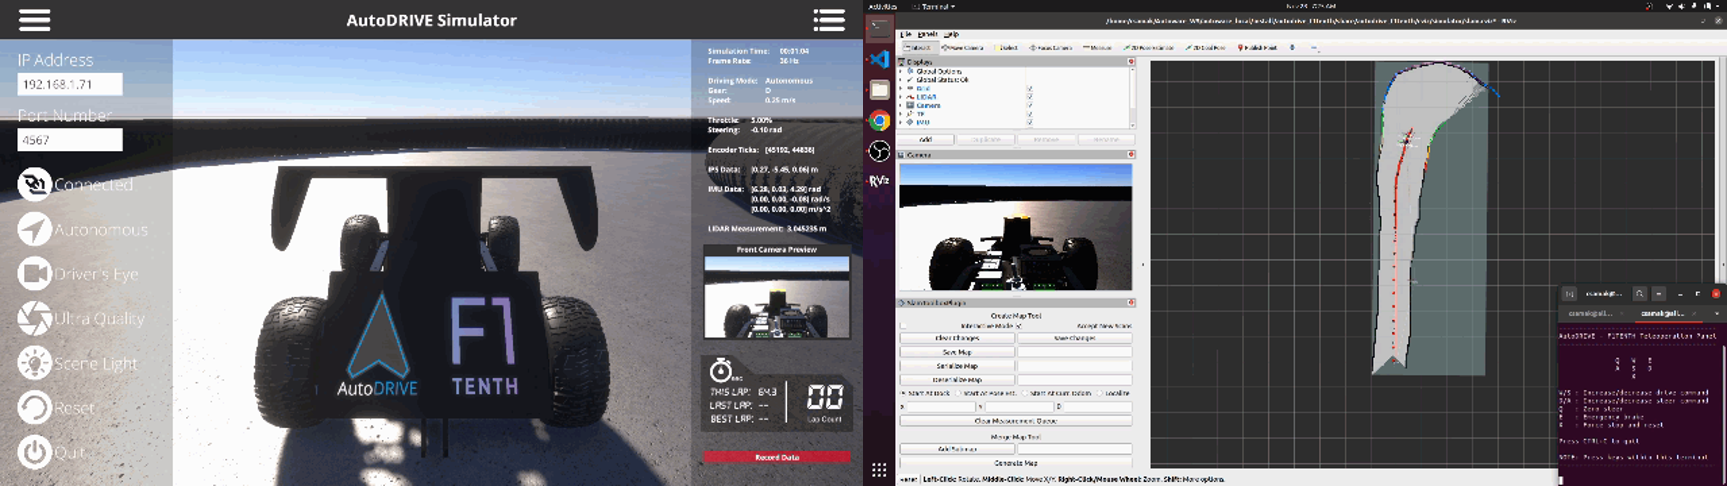
\includegraphics[width=\linewidth]{Figures/fig13.png}
    \caption{AutoDRIVE-F1TENTH-Autoware integration for autonomous racing ODD: AutoDRIVE Simulator demo for mapping an unknown racetrack using manual teleoperation.}
    \label{fig: figure13}
\end{figure}

\begin{figure}[H]
    \centering
    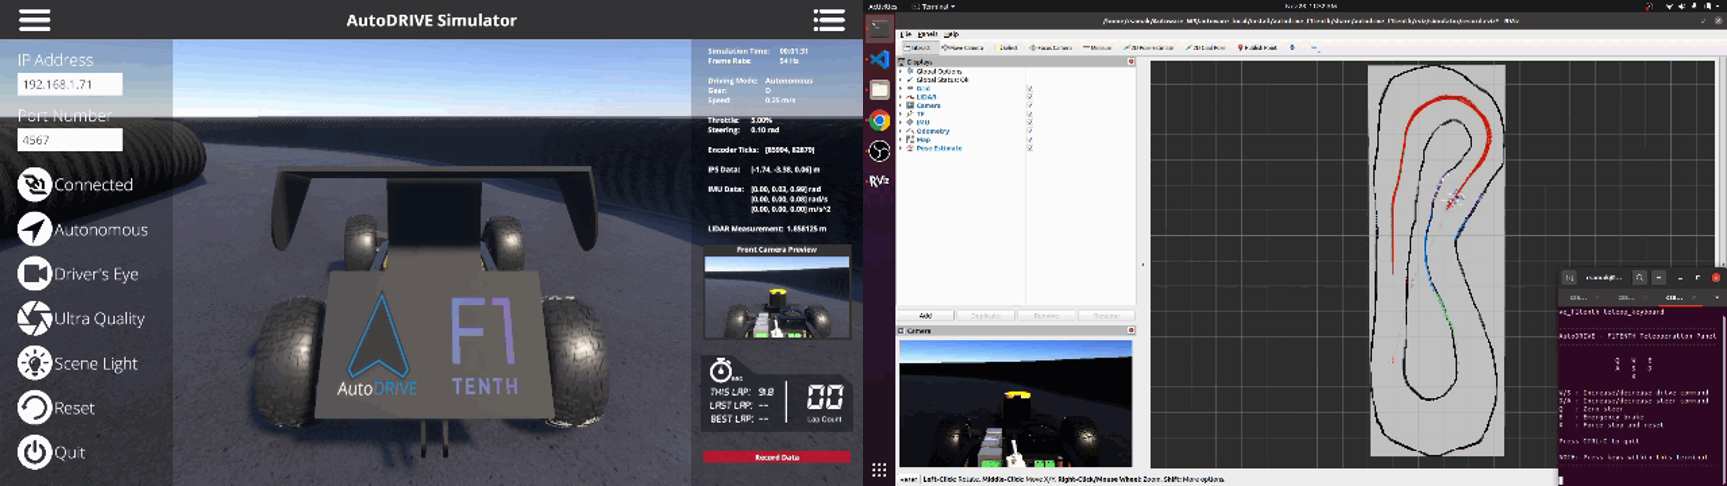
\includegraphics[width=\linewidth]{Figures/fig14.png}
    \caption{AutoDRIVE-F1TENTH-Autoware integration for autonomous racing ODD: AutoDRIVE Simulator demo for recording a trajectory using manual teleoperation.}
    \label{fig: figure14}
\end{figure}

\begin{figure}[H]
    \centering
    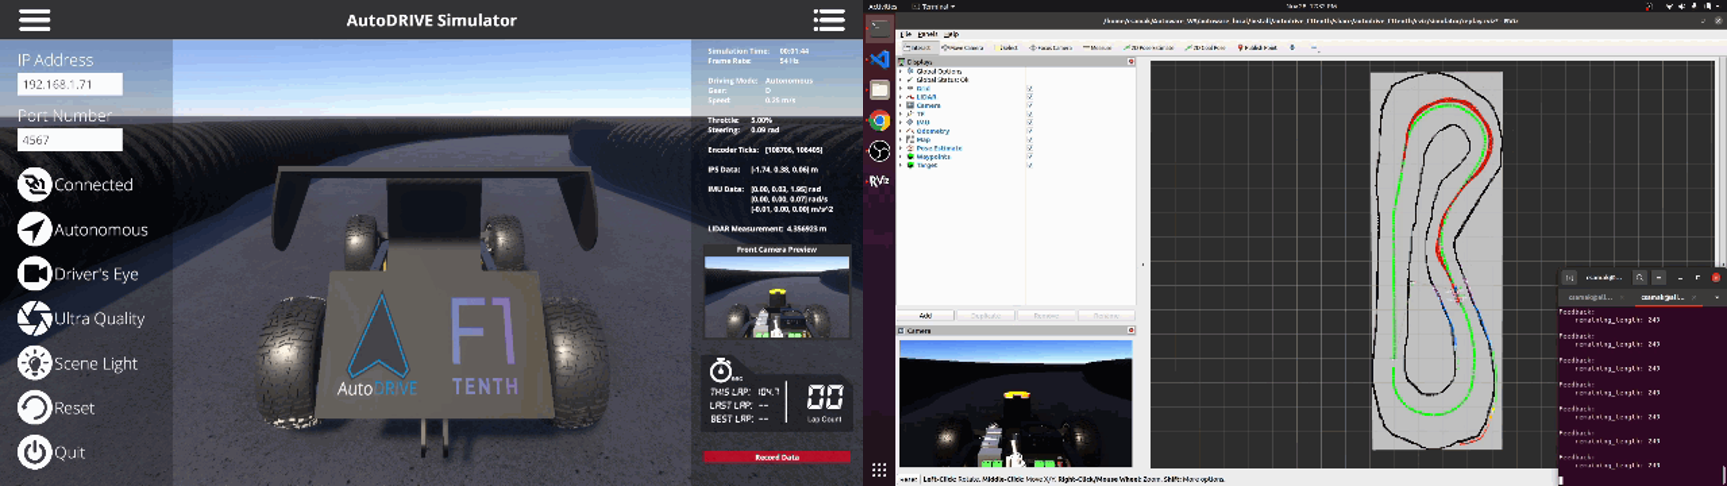
\includegraphics[width=\linewidth]{Figures/fig15.png}
    \caption{AutoDRIVE-F1TENTH-Autoware integration for autonomous racing ODD: AutoDRIVE Simulator demo for tracking the pre-recorded trajectory autonomously.}
    \label{fig: figure15}
\end{figure}

\begin{figure}[H]
    \centering
    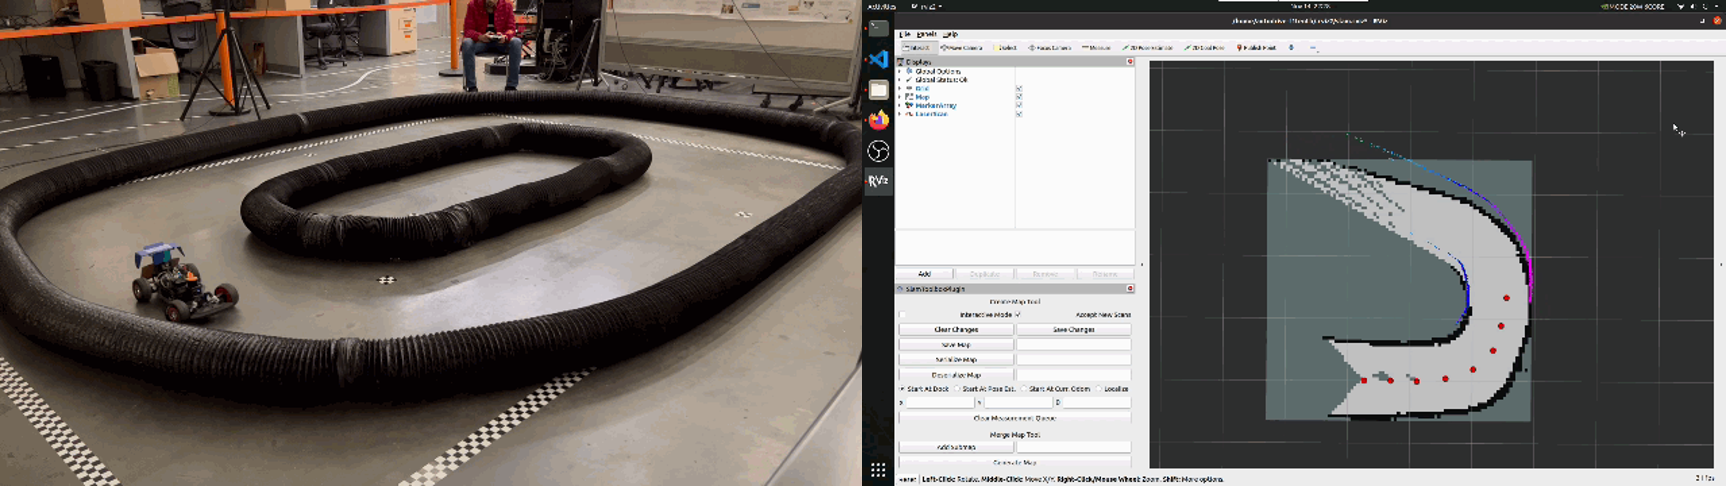
\includegraphics[width=\linewidth]{Figures/fig16.png}
    \caption{AutoDRIVE-F1TENTH-Autoware integration for autonomous racing ODD: Real-world demo for mapping an unknown racetrack using manual teleoperation.}
    \label{fig: figure16}
\end{figure}

\begin{figure}[H]
    \centering
    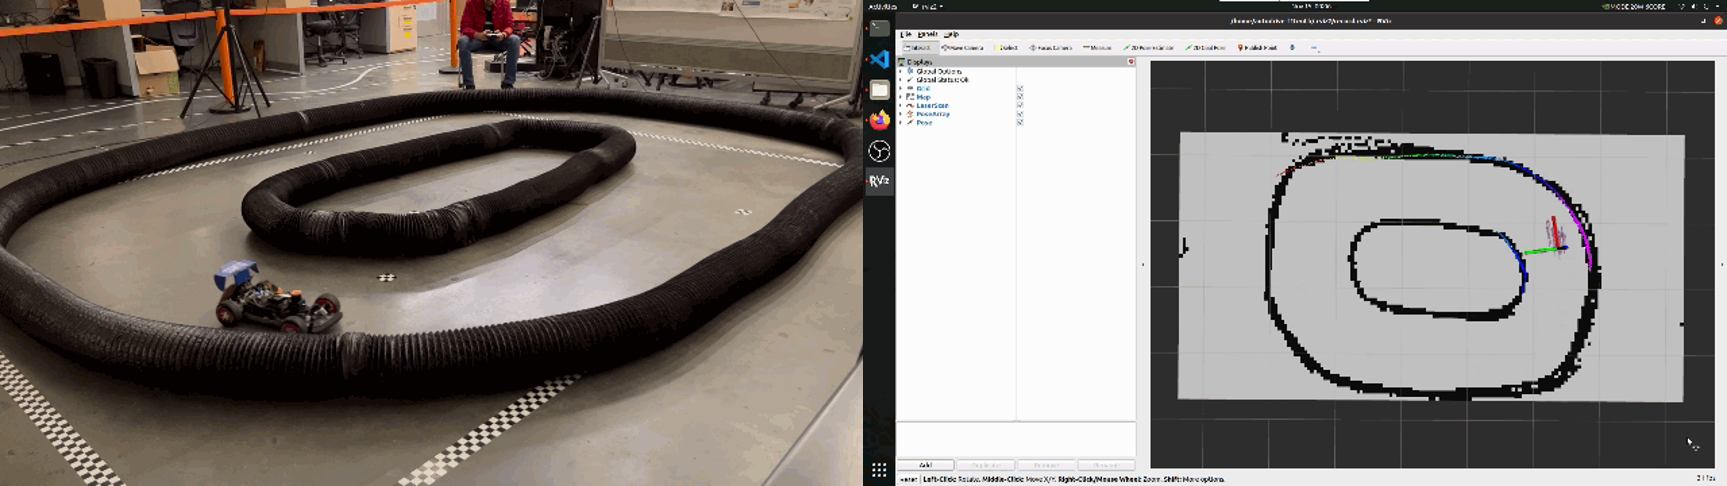
\includegraphics[width=\linewidth]{Figures/fig17.png}
    \caption{AutoDRIVE-F1TENTH-Autoware integration for autonomous racing ODD: Real-world demo for recording a trajectory using manual teleoperation.}
    \label{fig: figure17}
\end{figure}

\begin{figure}[H]
    \centering
    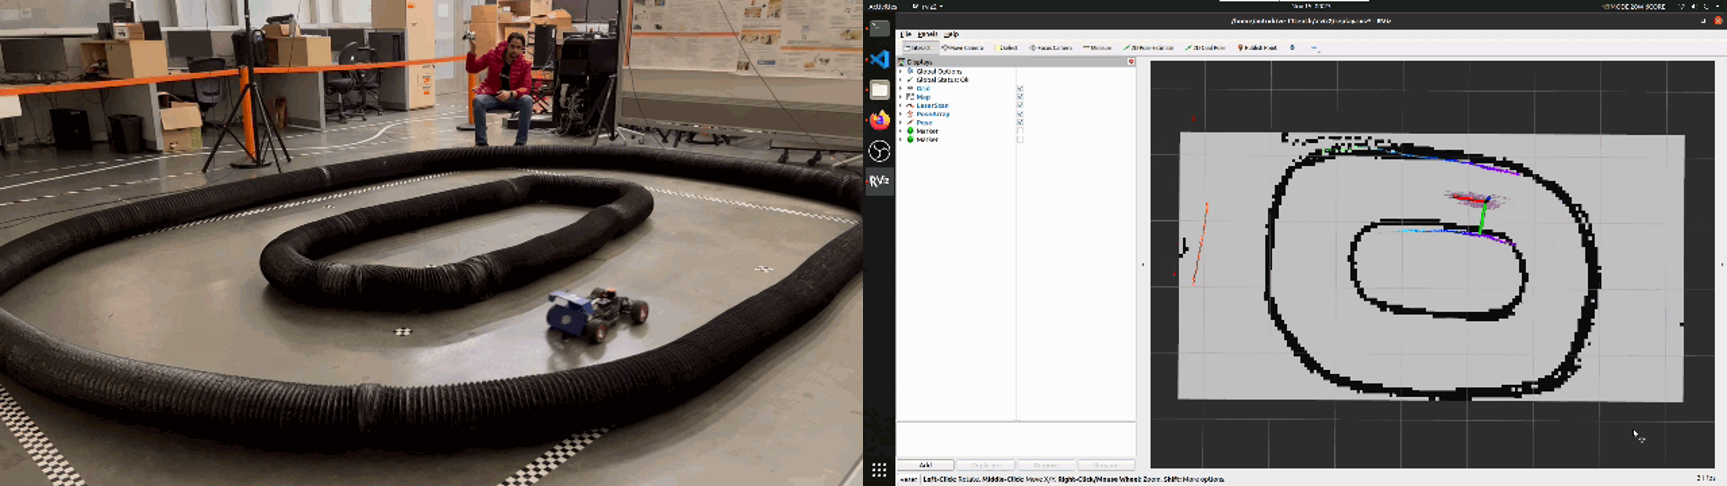
\includegraphics[width=\linewidth]{Figures/fig18.png}
    \caption{AutoDRIVE-F1TENTH-Autoware integration for autonomous racing ODD: Real-world demo for tracking the pre-recorded trajectory autonomously.}
    \label{fig: figure18}
\end{figure}

\hypertarget{Nigel}{%
\subsection{Nigel}\label{Nigel}}

\begin{figure}[H]
    \centering
    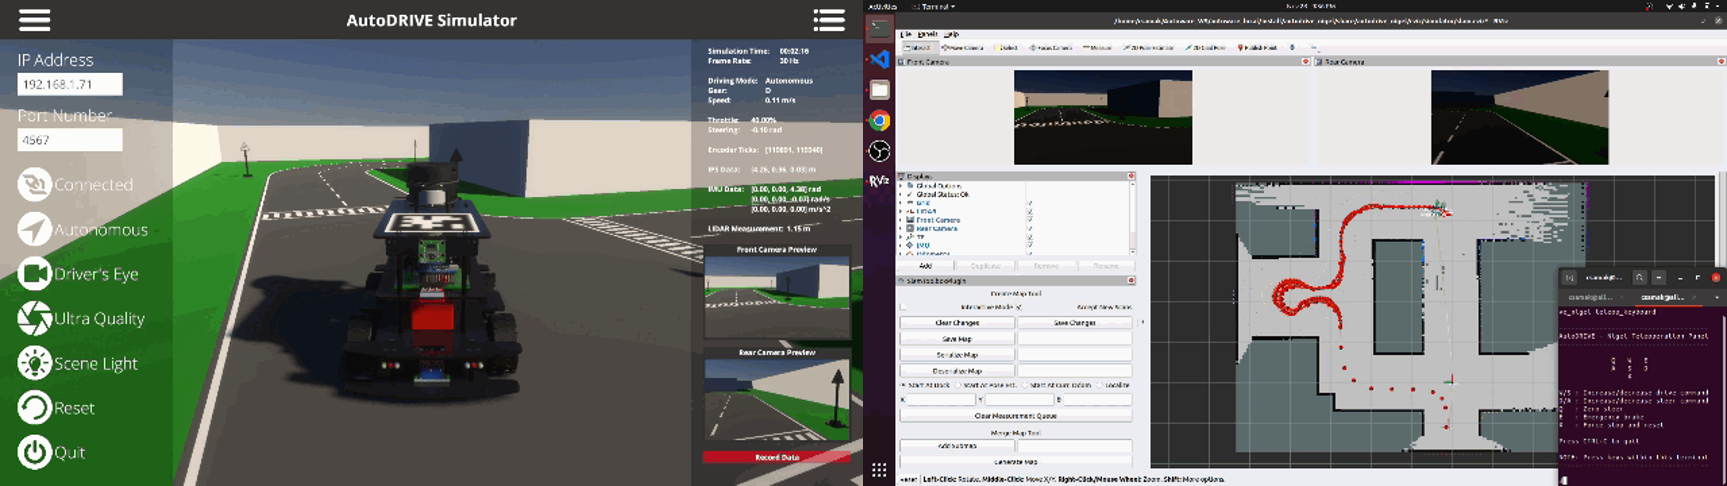
\includegraphics[width=\linewidth]{Figures/fig19.png}
    \caption{AutoDRIVE-Nigel-Autoware integration for autonomous valet parking ODD: AutoDRIVE Simulator demo for mapping an unknown environment using manual teleoperation.}
    \label{fig: figure19}
\end{figure}

\begin{figure}[H]
    \centering
    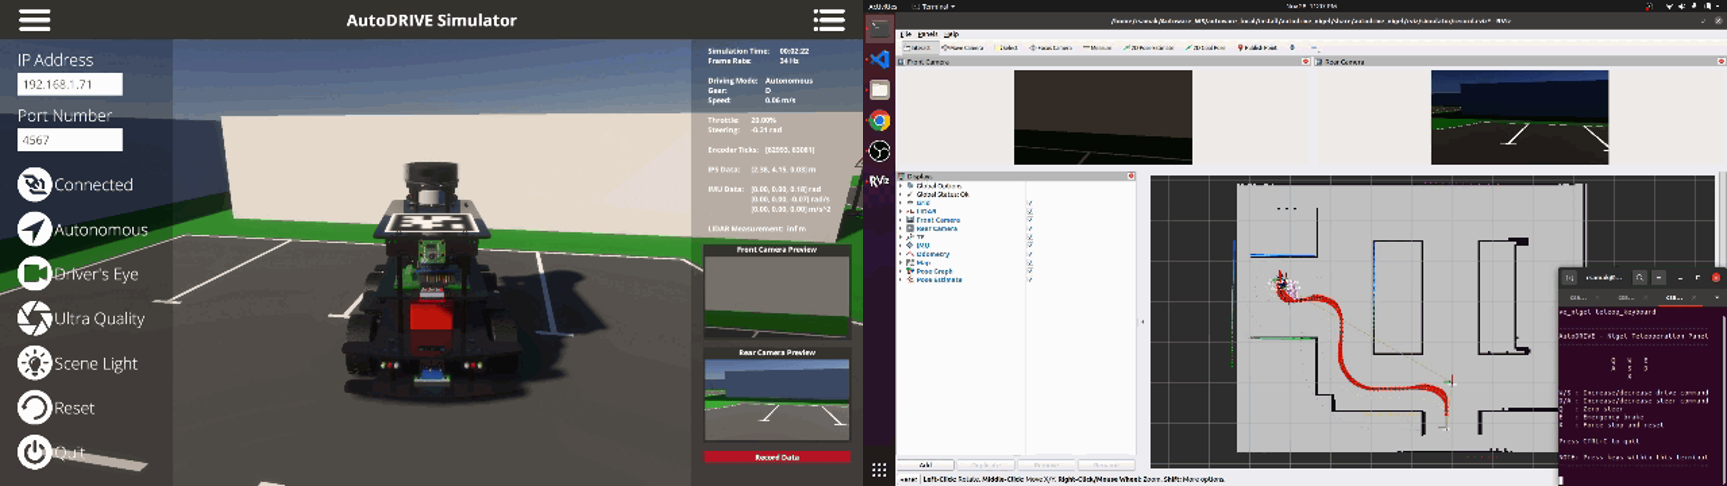
\includegraphics[width=\linewidth]{Figures/fig20.png}
    \caption{AutoDRIVE-Nigel-Autoware integration for autonomous valet parking ODD: AutoDRIVE Simulator demo for recording a trajectory using manual teleoperation.}
    \label{fig: figure20}
\end{figure}

\begin{figure}[H]
    \centering
    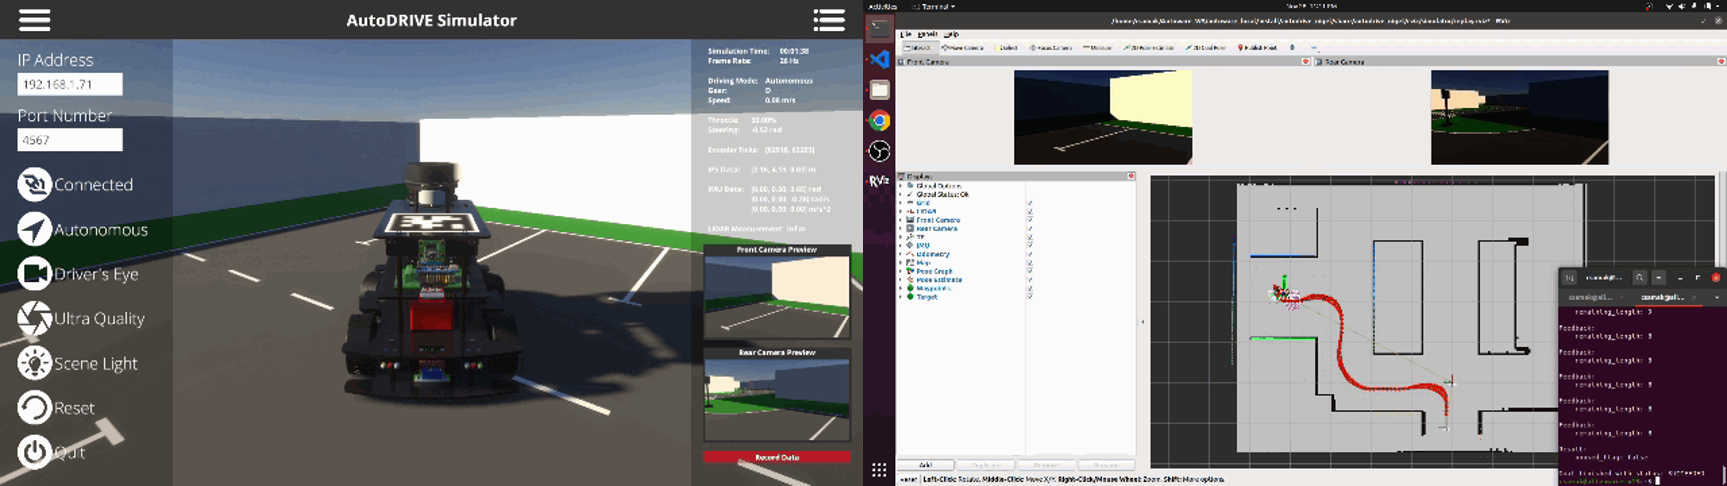
\includegraphics[width=\linewidth]{Figures/fig21.png}
    \caption{AutoDRIVE-Nigel-Autoware integration for autonomous valet parking ODD: AutoDRIVE Simulator demo for tracking the pre-recorded trajectory autonomously.}
    \label{fig: figure21}
\end{figure}

\begin{figure}[H]
    \centering
    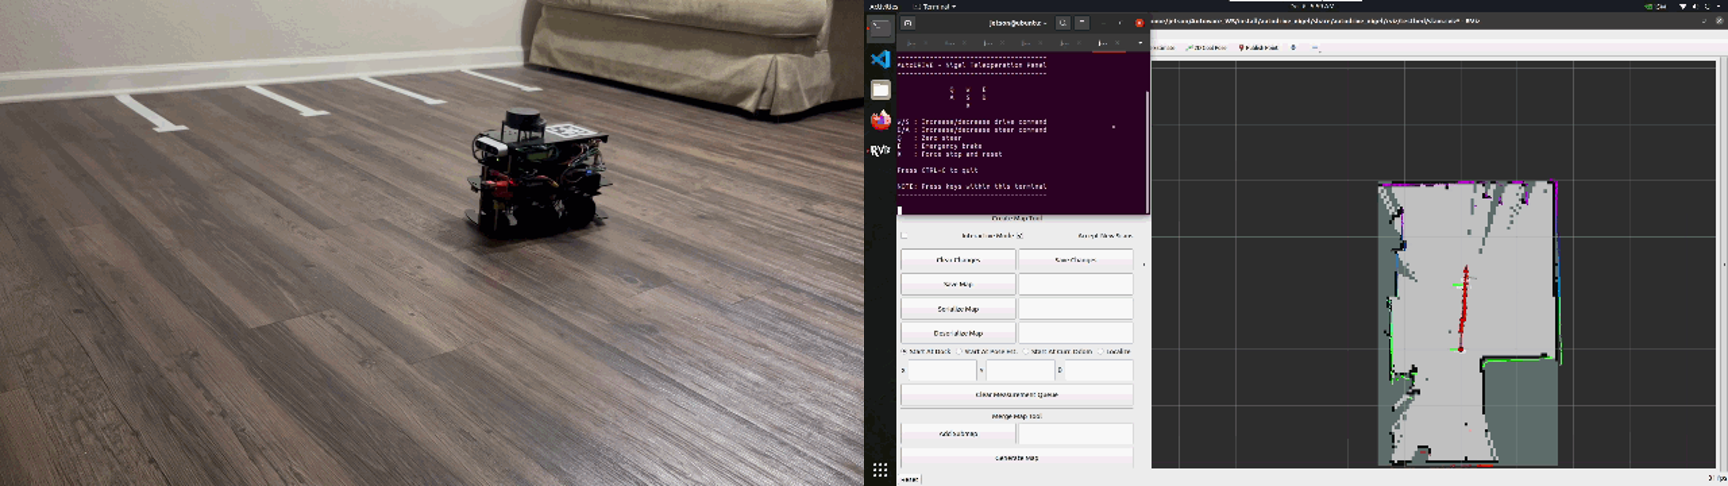
\includegraphics[width=\linewidth]{Figures/fig22.png}
    \caption{AutoDRIVE-Nigel-Autoware integration for autonomous valet parking ODD: Real-world demo for mapping an unknown environment using manual teleoperation.}
    \label{fig: figure22}
\end{figure}

\begin{figure}[H]
    \centering
    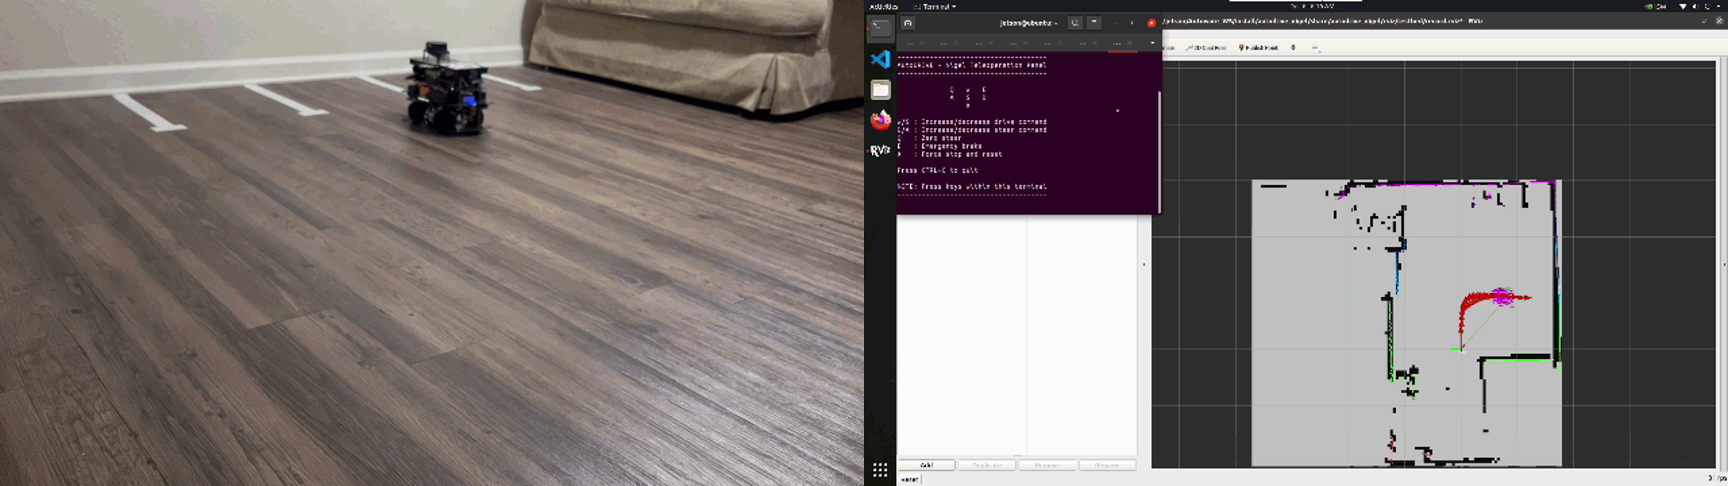
\includegraphics[width=\linewidth]{Figures/fig23.png}
    \caption{AutoDRIVE-Nigel-Autoware integration for autonomous valet parking ODD: Real-world demo for recording a trajectory using manual teleoperation.}
    \label{fig: figure23}
\end{figure}

\begin{figure}[H]
    \centering
    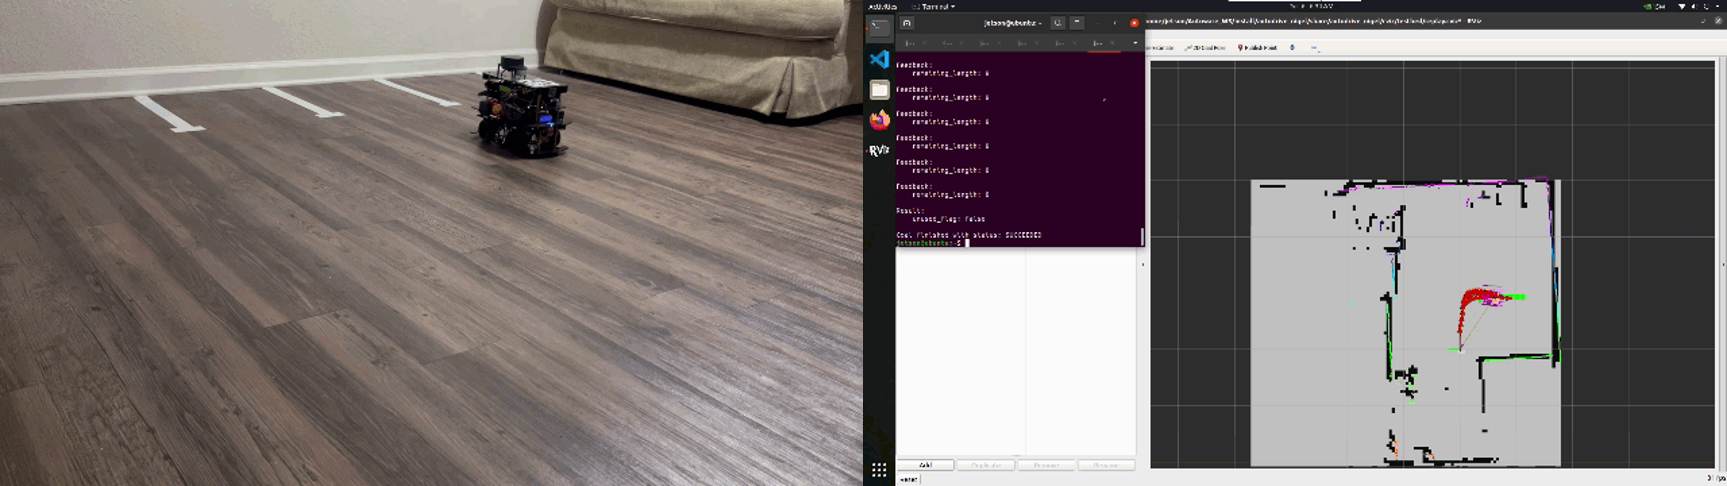
\includegraphics[width=\linewidth]{Figures/fig24.png}
    \caption{AutoDRIVE-Nigel-Autoware integration for autonomous valet parking ODD: Real-world demo for tracking the pre-recorded trajectory autonomously.}
    \label{fig: figure24}
\end{figure}

\hypertarget{Hunter SE}{%
\subsection{Hunter SE}\label{Hunter SE}}

\begin{figure}[H]
    \centering
    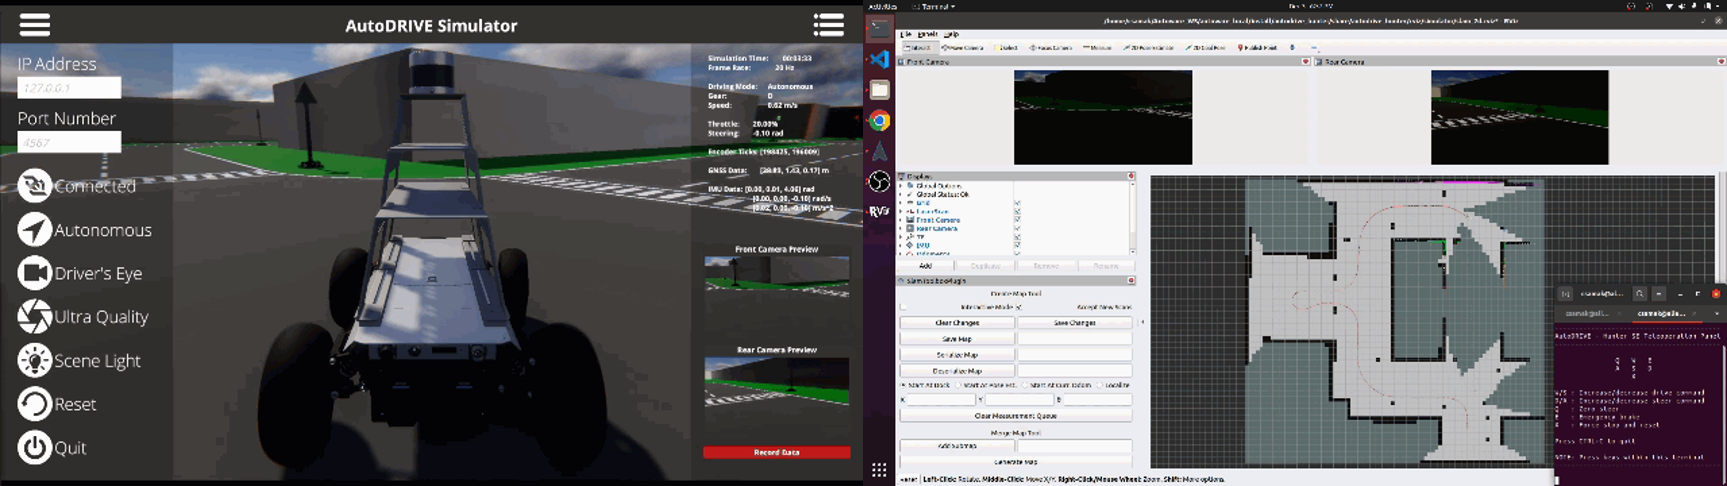
\includegraphics[width=\linewidth]{Figures/fig25.png}
    \caption{AutoDRIVE-HunterSE-Autoware integration for autonomous valet parking ODD: AutoDRIVE Simulator demo for mapping an unknown environment as a 2D binary occupancy grid (BOG) using manual teleoperation.}
    \label{fig: figure25}
\end{figure}

\begin{figure}[H]
    \centering
    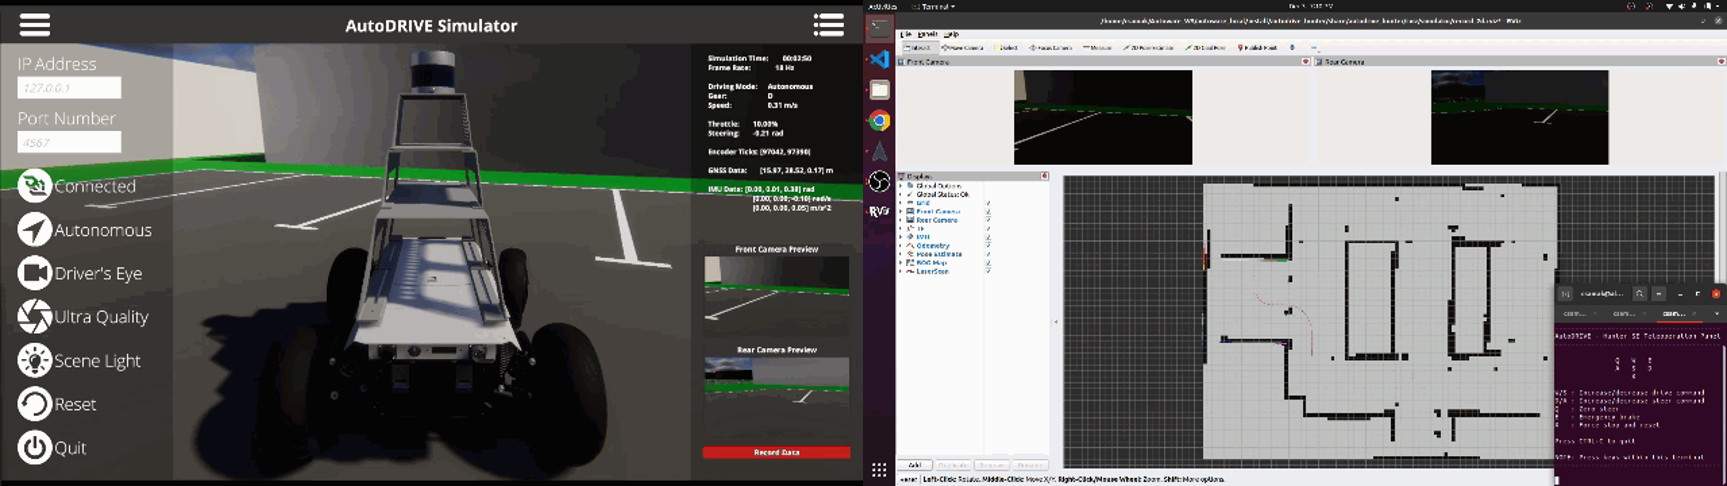
\includegraphics[width=\linewidth]{Figures/fig26.png}
    \caption{AutoDRIVE-HunterSE-Autoware integration for autonomous valet parking ODD: AutoDRIVE Simulator demo for recording a trajectory within the 2D binary occupancy grid (BOG) map using manual teleoperation.}
    \label{fig: figure26}
\end{figure}

\begin{figure}[H]
    \centering
    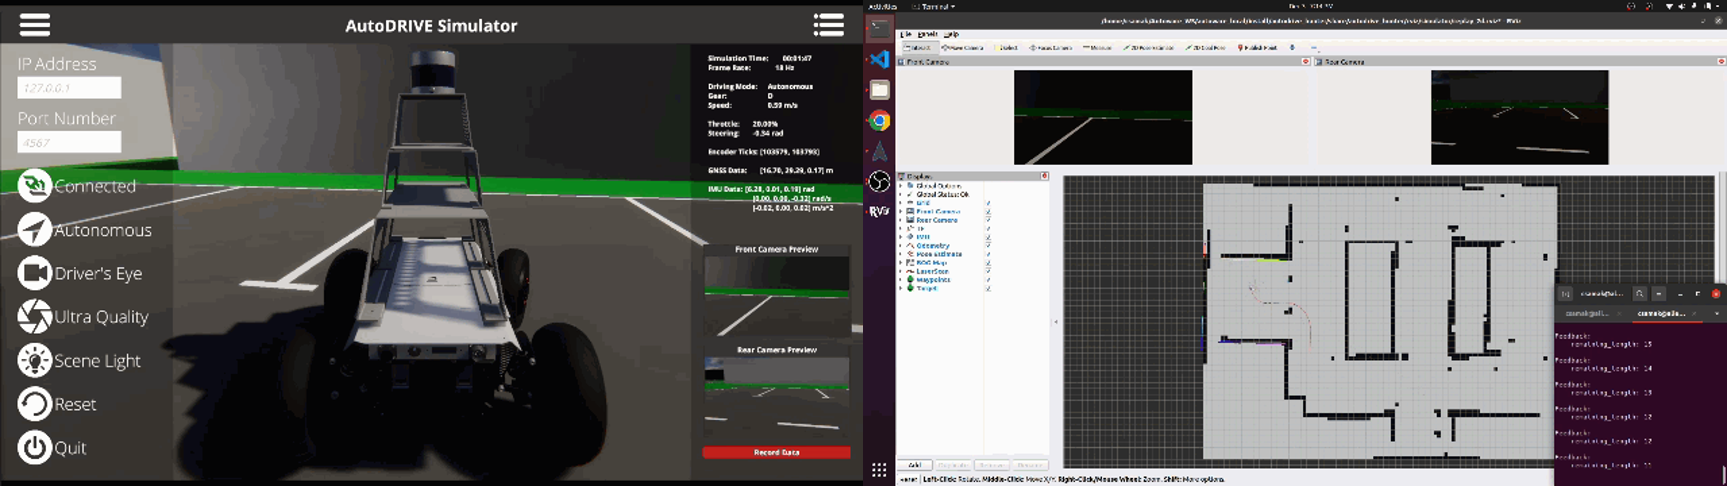
\includegraphics[width=\linewidth]{Figures/fig27.png}
    \caption{AutoDRIVE-HunterSE-Autoware integration for autonomous valet parking ODD: AutoDRIVE Simulator demo for tracking the pre-recorded trajectory autonomously within the 2D binary occupancy grid (BOG) map.}
    \label{fig: figure27}
\end{figure}

\begin{figure}[H]
    \centering
    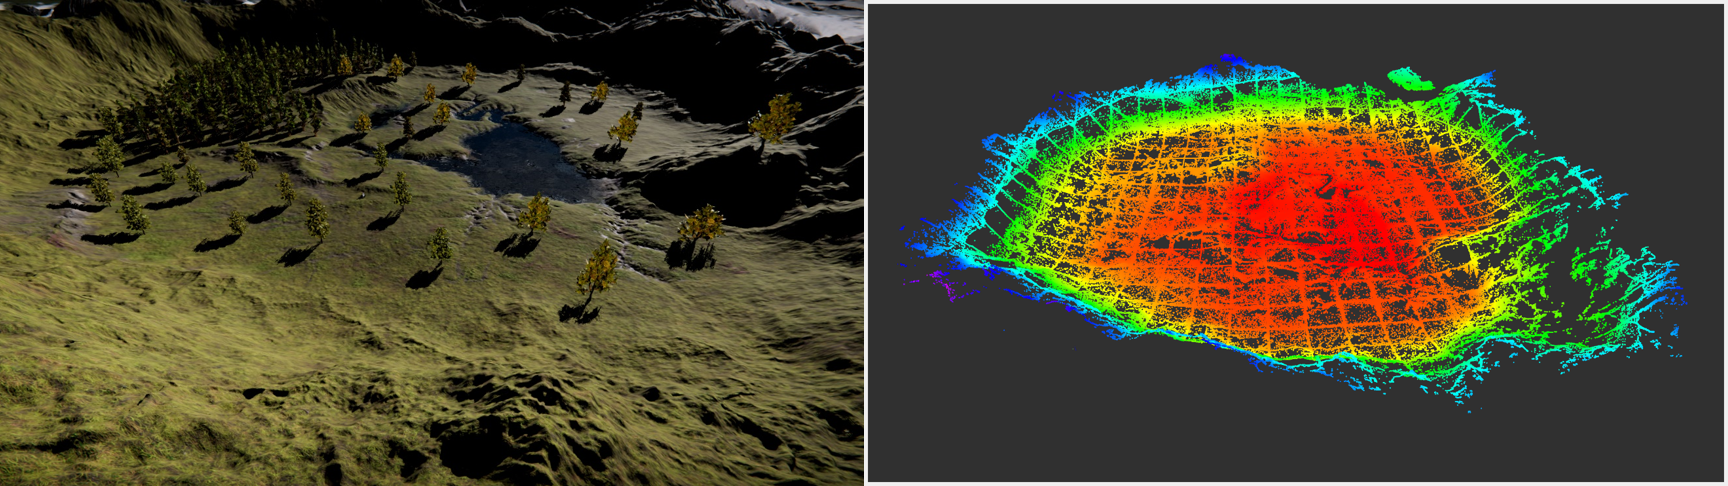
\includegraphics[width=\linewidth]{Figures/fig28.png}
    \caption{AutoDRIVE-HunterSE-Autoware integration for off-road exploration ODD: Generating and exporting 3D point cloud data (PCD) map directly from within AutoDRIVE Simulator using manual teleoperation.}
    \label{fig: figure28}
\end{figure}

\begin{figure}[H]
    \centering
    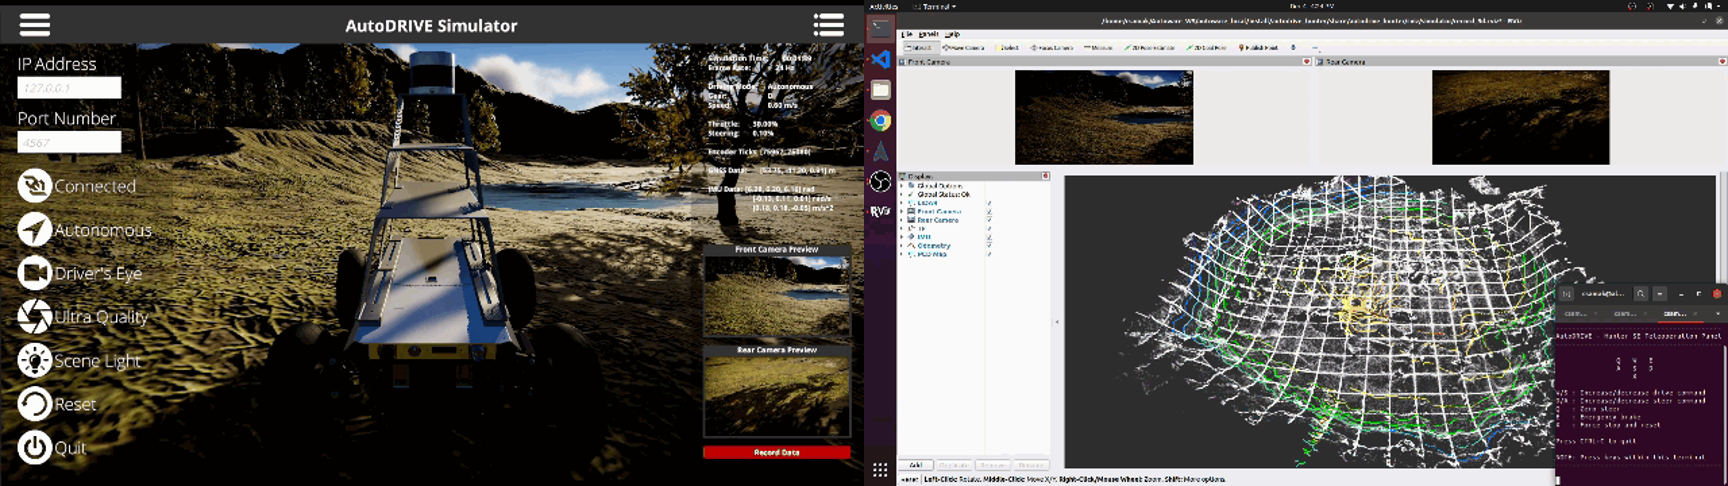
\includegraphics[width=\linewidth]{Figures/fig29.png}
    \caption{AutoDRIVE-HunterSE-Autoware integration for off-road exploration ODD: AutoDRIVE Simulator demo for recording a trajectory within the 3D point cloud data (PCD) map using manual teleoperation.}
    \label{fig: figure29}
\end{figure}

\begin{figure}[H]
    \centering
    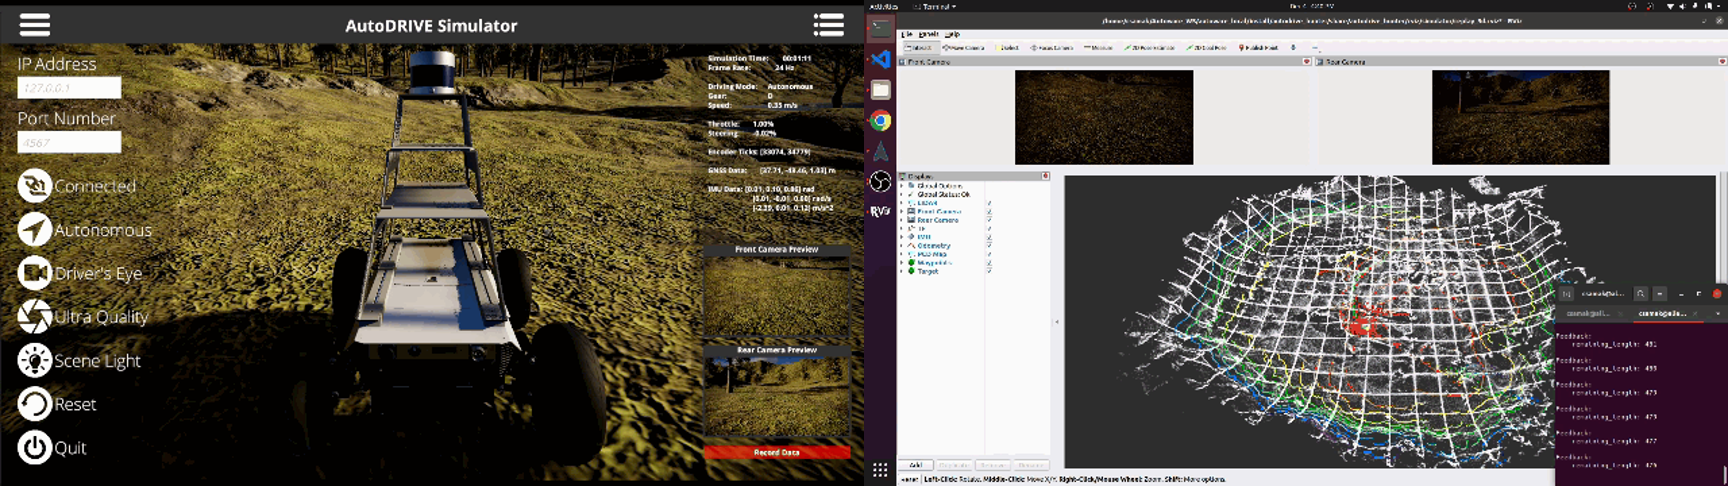
\includegraphics[width=\linewidth]{Figures/fig30.png}
    \caption{AutoDRIVE-HunterSE-Autoware integration for off-road exploration ODD: AutoDRIVE Simulator demo for tracking the pre-recorded trajectory autonomously within the 3D point cloud data (PCD) map.}
    \label{fig: figure30}
\end{figure}

\hypertarget{OpenCAV}{%
\subsection{OpenCAV}\label{OpenCAV}}

\begin{figure}[H]
    \centering
    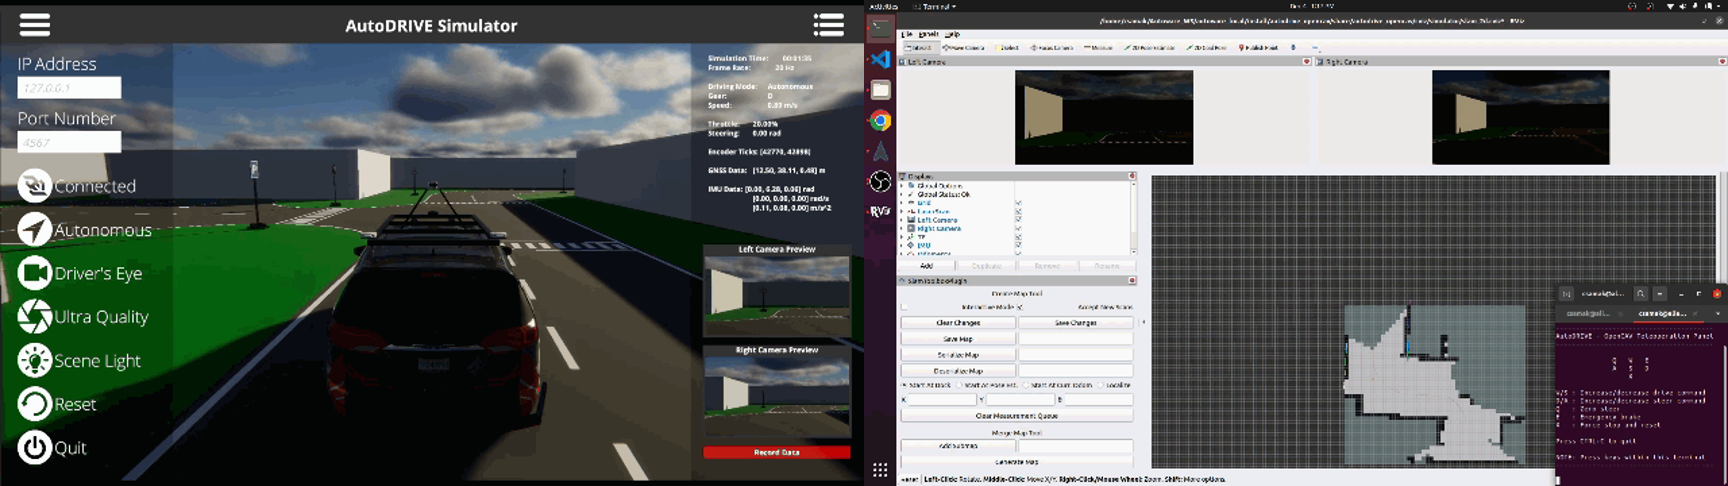
\includegraphics[width=\linewidth]{Figures/fig31.png}
    \caption{AutoDRIVE-OpenCAV-Autoware integration for autonomous valet parking ODD: AutoDRIVE Simulator demo for mapping an unknown environment as a 2D binary occupancy grid (BOG) using manual teleoperation.}
    \label{fig: figure31}
\end{figure}

\begin{figure}[H]
    \centering
    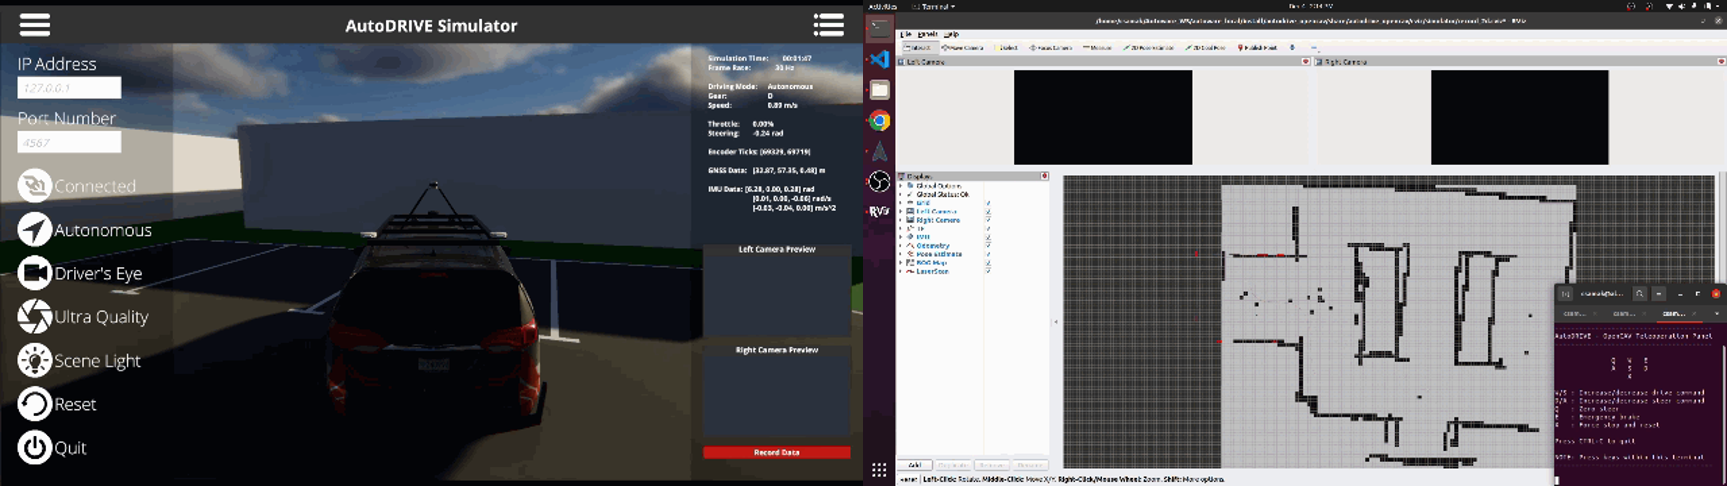
\includegraphics[width=\linewidth]{Figures/fig32.png}
    \caption{AutoDRIVE-OpenCAV-Autoware integration for autonomous valet parking ODD: AutoDRIVE Simulator demo for recording a trajectory within the 2D binary occupancy grid (BOG) map using manual teleoperation.}
    \label{fig: figure32}
\end{figure}

\begin{figure}[H]
    \centering
    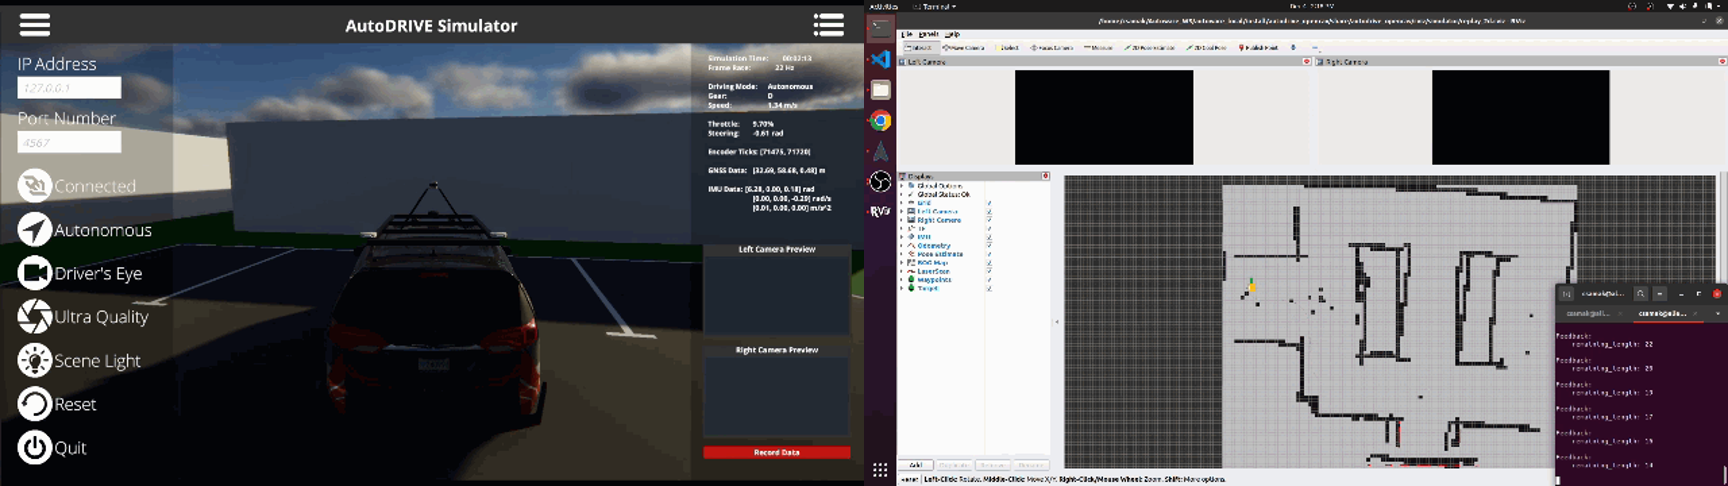
\includegraphics[width=\linewidth]{Figures/fig33.png}
    \caption{AutoDRIVE-OpenCAV-Autoware integration for autonomous valet parking ODD: AutoDRIVE Simulator demo for tracking the pre-recorded trajectory autonomously within the 2D binary occupancy grid (BOG) map.}
    \label{fig: figure33}
\end{figure}

\begin{figure}[H]
    \centering
    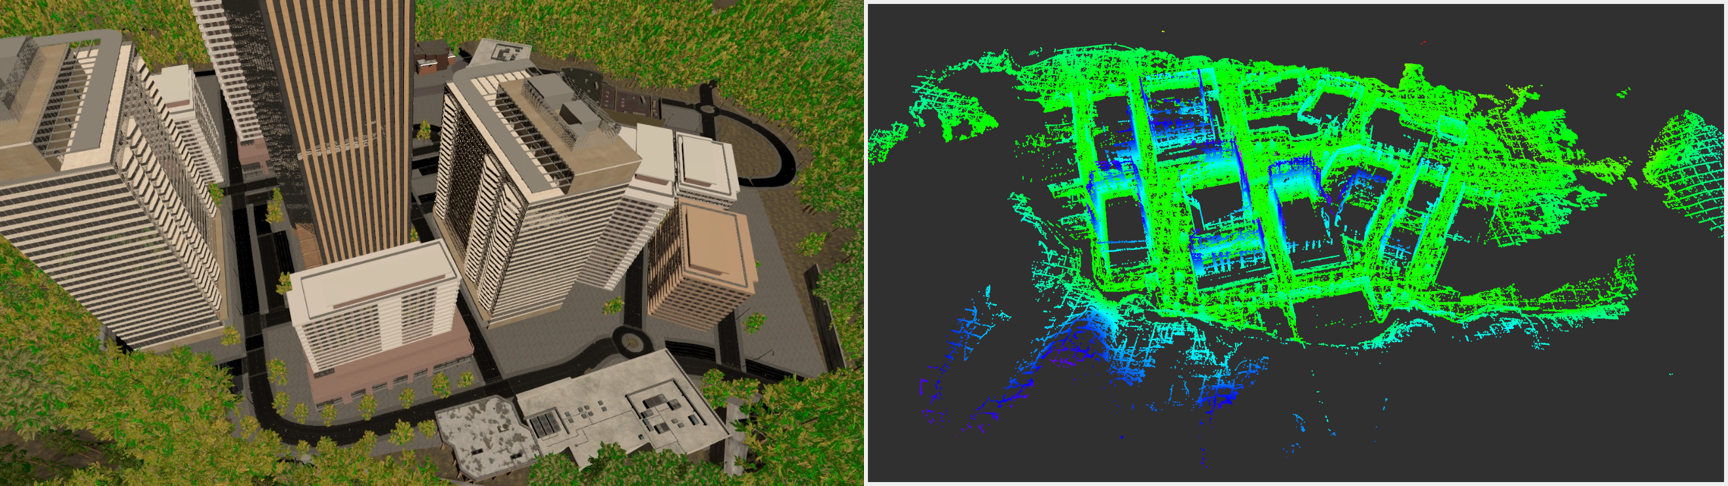
\includegraphics[width=\linewidth]{Figures/fig34.png}
    \caption{AutoDRIVE-OpenCAV-Autoware integration for autonomous valet parking ODD: Generating and exporting 3D point cloud data (PCD) map directly from within AutoDRIVE Simulator using manual teleoperation.}
    \label{fig: figure34}
\end{figure}

\begin{figure}[H]
    \centering
    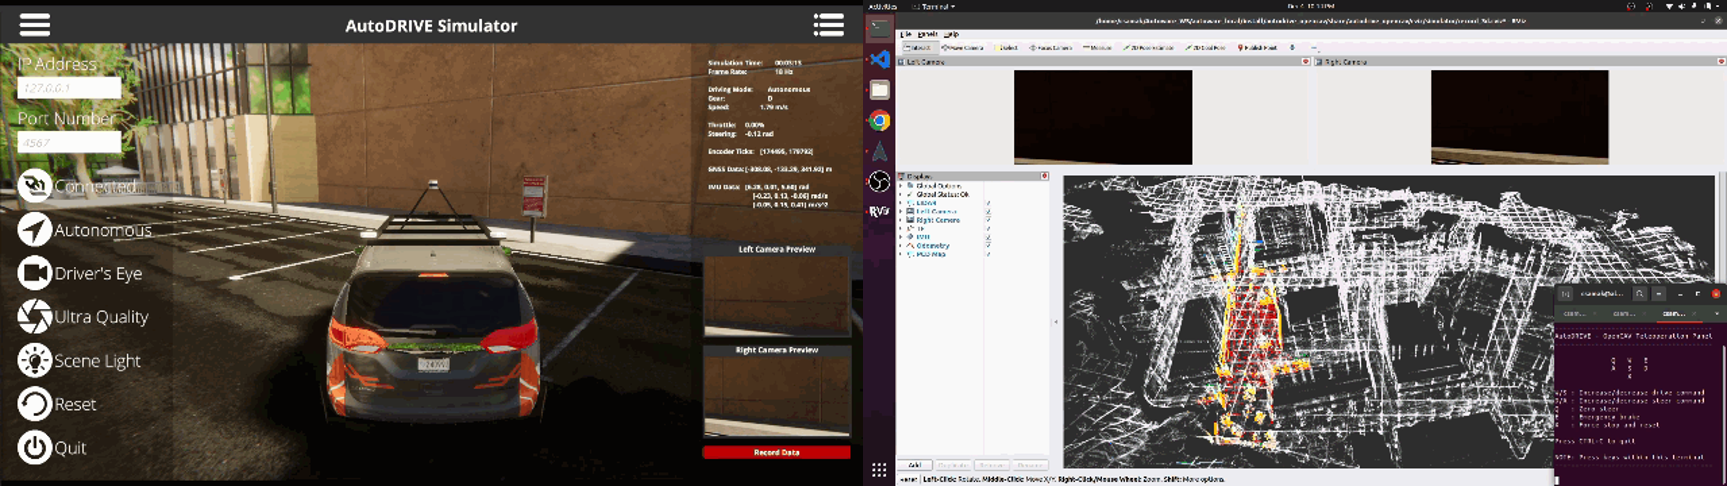
\includegraphics[width=\linewidth]{Figures/fig35.png}
    \caption{AutoDRIVE-OpenCAV-Autoware integration for autonomous valet parking ODD: AutoDRIVE Simulator demo for recording a trajectory within the 3D point cloud data (PCD) map using manual teleoperation.}
    \label{fig: figure35}
\end{figure}

\begin{figure}[H]
    \centering
    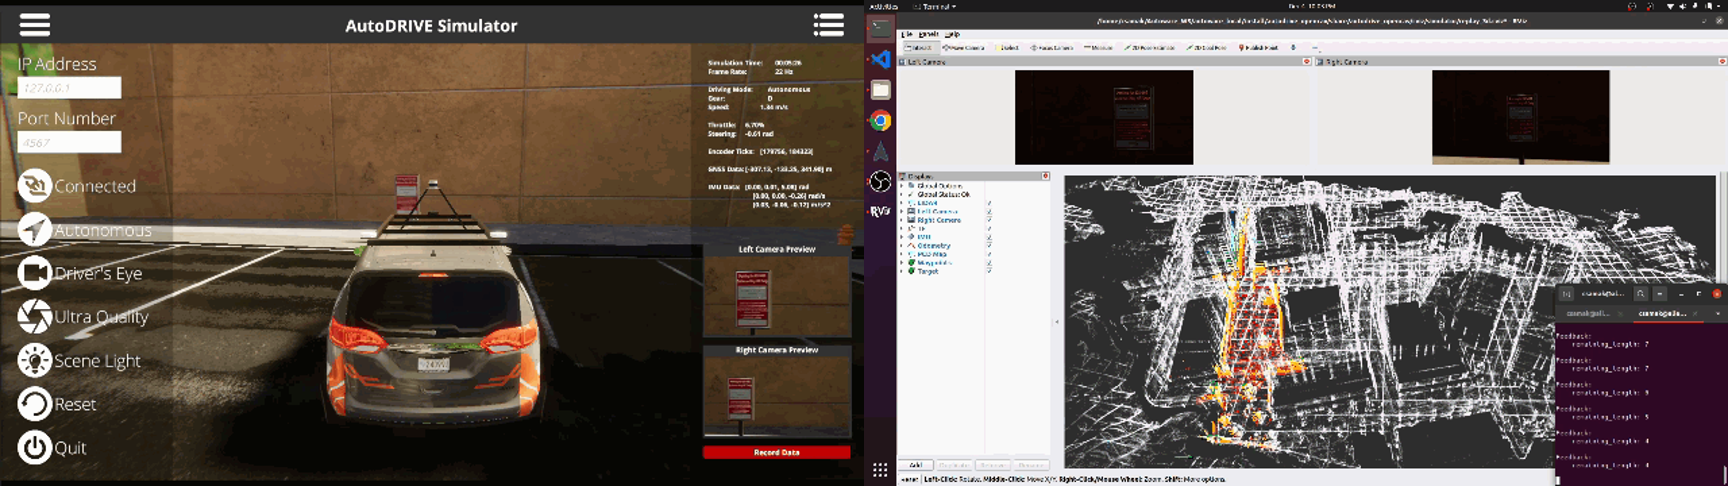
\includegraphics[width=\linewidth]{Figures/fig36.png}
    \caption{AutoDRIVE-OpenCAV-Autoware integration for autonomous valet parking ODD: AutoDRIVE Simulator demo for tracking the pre-recorded trajectory autonomously within the 3D point cloud data (PCD) map.}
    \label{fig: figure36}
\end{figure}